% Explain the implementation of the debugger and CLI

% Explain the first state where the debugger is not attach to the debugee
The debug thread has two main state that it changes between, the first state is when it is not attached to any debugee and is called DebugHandler.
The second state is when it is attach to the debugee which means that this state is where debugging can happen, it is called Debugger.
Going back to the fist state, its purpus is to await instructions to attach to the debugee and to recive configureation required for that to happen.
These configurations that the debuger requires is a path to the elf file, a path to the work directory of the code that should be debuged and lastly the type of chip.
When all these are configure the attach command can be used to attach to the microcontroller, all the other commands that require that the chip is attach can also be used to attach.


% Explain the second state where the debugger is attach to the debugee.
The debugger uses the library \emph{probe-rs} \cite{probe} to attach to the microcontroller and to interact with it.
Thus a lot of useful debuging features like stopping, continuing and setting hardware breakpoints is already given by the \emph{probe-rs} library.
The other features supported by the debugger uses the library \emph{rust-debug} together with the \emph{probe-rs} library.
But the two library are seprate so they never interact with each other, the figure \ref{fig:debugger} show how all of these parts interact.
The \emph{rust-debug} library as mention above and seen in the figure \ref{fig:debugger} is a library for retriving information form the \emph{DWRAF} sections in the \emph{ELF} file.
To get some of the information from the library values in the debugees memory and/or registers are needed.
Thus when the \emph{rust-debug} library gives a response to a requiese that it needs some specifig value the \emph{Debugger} \emph{Rust} struct can use \emph{probe-rs} to read those values.
Then those values can be sent in as a argument ot the \emph{rust-debug} library.
This repeats until the \emph{rust-debug} library returns the requested value or an error.


\begin{figure}[h]
    \centering
    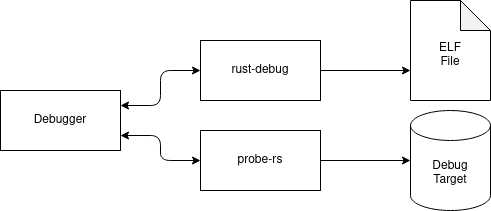
\includegraphics[width=1.0\textwidth]{debugger.png}
    \label{fig:debugger}
\end{figure}


% How the debugger handles request and events simultaneously.
To simontainisly handle incoming requiest form the user and events that happens in the debugee, the debugger polls the channel for incoming request and the state of the debugge.
To reduece the amount of polling of the state of the debugee the debugger has a boolean that keeps track of the state of the debugee.
This boolean is to track if the debugee is running or is stopped.
And because events can only ocur if the debugee is running the polling only needs to be done when it thinks the debugee is running.
Thus this is how the debugger can handle request from the user and near simontainisly handle events that happen in the debugee.


% How it handles request for stackframes and variables.
To improve of the preformance of the debugger the debugger stores the value of the stackframes every time they are callcualted.
This alows for fast repetetiv look up of stackframe information and variables.
The stored stackframe valuse are only stored when the debugee is stopped and are removed when the debugee starts.
Thus the wrong values will never be shown to the user.
Also another feature of the debugger is that if the value of a variable is requeste the debugger will retive all the stackframes instad and then search for the requested variable.
This simplifies the implementation a lot and will also make the debugger faster when repeted request are made.

